% \documentclass[twocolumn]{article}
\documentclass[runningheads]{llncs}

\usepackage[brazil]{babel}
\usepackage[latin1,utf8]{inputenc}
\usepackage{pifont}

%% Math
\usepackage{mathtools}
\usepackage{amsmath}
\usepackage{commath}

\usepackage{amsfonts}% revise se precisa ou não
\usepackage{nccmath}% revise se precisa ou não

\usepackage[numbers]{natbib}
\usepackage{multirow}
\usepackage{makecell}
\usepackage{graphicx}

\usepackage{listings}
\usepackage{float}
\usepackage{enumitem}

\usepackage{wasysym}
\usepackage{resizegather}

\renewcommand{\lstlistingname}{Código}
\renewcommand{\lstlistlistingname}{Lista de \lstlistingname s}

%\definecolor{codegreen}{rgb}{0,0.6,0}
%\definecolor{codegray}{rgb}{0.85,0.85,0.85}
%\definecolor{codepurple}{rgb}{0.58,0,0.82}
%\definecolor{codeblack}{rgb}{0,0,0}

\lstdefinelanguage{JavaScript}{
  keywords={typeof, new, true, false, catch, function, return, null, catch, switch, var, if, in, while, do, else, case, break},
  %keywordstyle=\color{blue}\bfseries,
  ndkeywords={class, export, boolean, throw, implements, import, this},
  %ndkeywordstyle=\color{codegray}\bfseries,
  %identifierstyle=\color{black},
  sensitive=false,
  comment=[l]{//},
  morecomment=[s]{/*}{*/},
  %commentstyle=\color{purple}\ttfamily,
  %stringstyle=\color{red}\ttfamily,
  morestring=[b]',
  morestring=[b]"
}

\lstdefinestyle{codigo}{
    backgroundcolor=\color{codegray},   
    commentstyle=\color{codegreen},
    keywordstyle=\color{magenta},
    numberstyle=\tiny\color{codeblack},
    stringstyle=\color{codepurple},
    basicstyle=\ttfamily\footnotesize,
    breakatwhitespace=false,         
    breaklines=true,                 
    captionpos=b,                    
    keepspaces=true,                 
    numbers=left,                    
    numbersep=5pt,                  
    showspaces=false,                
    showstringspaces=false,
    showtabs=false,                  
    tabsize=4
}

\lstset{style=codigo}

\DeclarePairedDelimiter{\round}\lfloor\rceil
\newcommand\citetxt[1]{%
  \citeauthor{#1}~(\citeyear{#1})}
\newcommand\citepar[1]{%
  (\citeauthor{#1}, \citeyear{#1})} 
  


%https://tex.stackexchange.com/q/151984/7561
\DeclarePairedDelimiterX{\infdivx}[2]{(}{)}{%
  #1\;\delimsize\|\;#2%
}
\newcommand{\kl}{\operatorname{KL}\infdivx}
\newcommand{\skl}{\operatorname{SKL}\infdivx}

% https://tex.stackexchange.com/questions/23773/a-centered-plus-minus-symbol
\newcommand{\rpm}{\raisebox{.2ex}{$\scriptstyle\pm$}}

% https://tex.stackexchange.com/a/141685/7561
\newcommand\givenbase[1][]{\:#1\lvert\:}
\let\given\givenbase

% https://tex.stackexchange.com/a/171959/7561
\newcommand\reallywidehat[1]{\ThisStyle{%
    \setbox0=\hbox{$\SavedStyle#1$}%
    \stackengine{-1.0\ht0+.5pt}{$\SavedStyle#1$}{%
      \stretchto{\scaleto{\SavedStyle\mkern.15mu\char'136}{1.5\wd0}}{1.4\ht0}%
    }{O}{c}{F}{T}{S}%
}}
\newcommand{\hkl}{\widehat{\operatorname{KL}}\infdivx}

% Conditional independence symbol
% https://tex.stackexchange.com/questions/218631/symbol-for-not-conditionally-independent/
\newcommand{\CI}{\mathrel{\perp\mspace{-10mu}\perp}}

% declare my argmin and argmax operators
% https://tex.stackexchange.com/a/5255/7561
\DeclareMathOperator*{\argmax}{arg\,max}
\DeclareMathOperator*{\argmin}{arg\,min}

% declaring an expectation operator to behave like sum
% https://tex.stackexchange.com/a/23436/7561
\makeatletter
\DeclareRobustCommand\bigop[1]{%
  \mathop{\vphantom{\sum}\mathpalette\bigop@{#1}}\slimits@
}
\newcommand{\bigop@}[2]{%
  \vcenter{%
    \sbox\z@{$#1\sum$}%
    \hbox{\resizebox{\ifx#1\displaystyle.9\fi\dimexpr\ht\z@+\dp\z@}{!}{$\m@th#2$}}%
  }%
}
\makeatother

% Keywords command
\providecommand{\keywords}[1]
{
  \small	
  \textbf{\textit{Keywords ---}} #1
}
\providecommand{\palavraschave}[1]
{
  \small	
  \textbf{\textit{Palavras-chave ---}} #1
}

%\newcommand{\E}{\DOTSB\bigop{\mathbb{E}}}
\DeclareMathOperator*{\E}{\mathbb{E}}

% redefining \times operator
\let\oldtimes\times
\def\times{{\mkern1mu\oldtimes\mkern1mu}}



\usepackage{subfigure}
\newcommand{\cmark}{\ding{51}}%

%\DeclarePairedDelimiter\abs{\lvert}{\rvert}%
%\DeclarePairedDelimiter\norm{\lVert}{\rVert}%
\DeclarePairedDelimiter\product{\langle}{\rangle}%

\usepackage{cellspace}
\setlength\cellspacetoplimit{6pt}
\setlength\cellspacebottomlimit{4pt}

%% Units
\usepackage{siunitx}

%% Tables
\usepackage{booktabs}


% Para acrescentar comentários ao PDF descomente:
\usepackage
%  [pdfauthor={nome do autor},
%   pdftitle={titulo},
%   pdfkeywords={palavra-chave, palavra-chave},
%   pdfproducer={Latex with hyperref},
%   pdfcreator={pdflatex}]
{hyperref}

% Os cores podem ser mudados
\hypersetup{
%  linkcolor={red!50!black},
%  citecolor={blue!50!black},
%  urlcolor={blue!80!black}
}

\usepackage{url}
\usepackage{breakurl}
% \usepackage[breaklinks]{hyperref}

\def\UrlBreaks{\do\/\do-\do\_}

\title{\textit{Workflow} semi-autonômico para aplicações de \textit{Machine Learning} utilizando métricas de \textit{Fairness}}
%\titlerunning{\textit{Workflow} semi-autonômico para aplicações de \textit{Machine Learning} utilizando métricas de \textit{Fairness}}

\author{Thales Eduardo Nazatto\textsuperscript{1}, Cecília Mary Fischer Rubira\textsuperscript{2}, Leonardo Montecchi\textsuperscript{3}}
\institute{
	\textsuperscript{1} UNICAMP, Campinas, Brasil, tenazatto@gmail.com
	\\
	\textsuperscript{2} UNICAMP, Campinas, Brasil, cmrubira@ic.unicamp.br
	\\
	\textsuperscript{3} NTNU, Trondheim, Noruega, leonardo.montecchi@ntnu.no\\[2ex]
}

\date{
	\textsuperscript{1} UNICAMP, Campinas, Brasil, tenazatto@gmail.com
	\\
	\textsuperscript{2} UNICAMP, Campinas, Brasil, cmrubira@ic.unicamp.br
	\\
	\textsuperscript{3} NTNU, Trondheim, Noruega, leonardo.montecchi@ntnu.no\\[2ex]
	\today
}

%\authorrunning{Thales Eduardo Nazatto, Cecília Mary Fischer Rubira, Leonardo Montecchi}

\begin{document}

\maketitle

\begin{abstract}
O uso de Aprendizado de Máquina (ML) envolvendo grandes volumes de dados vem crescendo conforme nossa sociedade migra processos manuais de trabalho para soluções digitais e necessita de tomadas de decisão mais rápidas e assertivas, mas, devido a barreiras éticas e legais, métricas usadas inicialmente para definir a eficácia de um algoritmo se mostraram limitadas para medir vieses que refletem a sociedade de maneira que não era esperada pelos desenvolvedores da solução. Para resolver tal problema, novos algoritmos foram desenvolvidos e um novo conjunto de métricas, denominado como métricas de Fairness, é utilizado para determinar um equilíbrio aos grupos que sofrem discriminações. Entretanto, com estas novas descobertas, aumenta-se a complexidade da análise do Cientista de Dados para obter modelos com os melhores resultados. Este artigo foca no tema de Aprendizado de Máquina do ponto de vista da Engenharia de Software, apresentando uma solução para aplicações de \textit{Machine Learning} que pode ser executado de maneira autônoma sem a necessidade de experimentar uma grande quantidade de técnicas e pode ser mais assertivo em encontrar opções mais otimizadas para diferentes contextos, utilizando um \textit{Workflow} que possui uma diversa gama de algoritmos já implementados e utiliza a arquitetura MAPE-K para determinar qual possui o melhor balanceamento. Foram realizados diversos estudos de caso para determinar se o MAPE-K pode ser viável na resolução destes problemas e se a solução implementada é extensível sem grandes esforços, possibilitando um maior uso de algoritmos. Diante deste contexto, foi notado que a solução pode facilitar caminhos realizados pelo Especialista de ML, possibilitando estudos de Engenharia de Software em aplicações com o uso responsável de dados.

\keywords{\textit{Workflow}, \textit{Machine Learning}, Inteligência Artificial, Computação Autônoma, Métricas de \textit{Fairness}}
\end{abstract}

\section{Introdução}

Técnicas de Inteligência Artificial e Aprendizado de Máquina já são utilizadas há bastante tempo no ramo da Computação. Ramos como robótica e jogos são grandes exemplos, dada a necessidade nos mesmos de automatizar comportamentos que seriam tidos como triviais para um ser humano. Entretanto, nos últimos anos ocorreu um crescimento no uso dessas tecnologias em aplicações tradicionais, devido principalmente à grande quantidade de dados processada diariamente pelas empresas e pela quantidade de processamento disponível a custos baixos. Diferentes perfis podem traçados com esses dados e usar soluções de IA gera tomadas de decisão mais assertivas com o objetivo de melhorar a experiência de usuário e corrigir problemas. Porém, um efeito colateral comum nestas soluções é a exposição de vieses que, embora sejam vistos como não-intencionais pelos desenvolvedores por ter a possibilidade de ser um \textit{outlier} no modelo treinado, refletem preconceitos escancarados da sociedade atual. Uma entrada de dados enviesada resulta em um algoritmo que realiza discriminações em sua classificação~\citep{Buolamwini_2018}, e uma vez que as métricas utilizadas para medir a qualidade de um modelo final são geralmente baseadas em acurácia, precisão e recall, discriminações não são facilmente percebidas por tais métricas.

Devido a esse problema, é possível estabelecer métricas para determinar o quão o modelo está preparado para dados sensíveis~\citep{Begley_2021}, termo que é conhecido como \textit{Fairness}. Com a evolução das pesquisas na comunidade acadêmica, foram descobertos algoritmos para redução dos vieses presentes nos conjuntos de dados, como \textit{Reweighing}~\citep{Kamiran_2011}, \textit{Adversarial Debiasing}~\citep{Zhang_2018} e \textit{Reject Option Classification}~\citep{Kamiran_2012}. Por consequência, ocorre melhora nas métricas em questão, mas pode desfavorecer métricas que já são amplamente utilizadas como garantia de um bom modelo desenvolvido com técnicas de Aprendizado de Máquina.

Para este determinado contexto, foi desenvolvida uma estrutura de \textit{Workflow} para aplicações de \textit{Machine Learning} que é manuseada pelo Cientista de Dados de forma semi-autônoma, focada em dois objetivos principais:

\begin{itemize}
\item Facilitar a criação de modelos justos e confiáveis com a automatização da escolha dos algoritmos, cuja complexidade aumenta com a escolha dos algoritmos a serem utilizados e suas execuções nas etapas corretas do processo, onde eles foram escolhidos para atuar.
\item Estabelecer um balanceamento entre métricas para avaliar bons modelos com métricas para avaliar modelos justos.
\end{itemize}

Esta estrutura é dividida em 5 módulos: Engenharia de Dados, \textit{Workflow} de ML, Gerenciador Autonômico, Backend e Interface. Para a Engenharia de Dados, foram realizadas modificações nos conjuntos de dados German Credit Dataset~\citep{ucigerman_2021} e Lendingclub Dataset~\citep{lendingclub_2022} para serem adequados ao uso do \textit{workflow}. Para o desenvolvimento e estruturação do \textit{workflow}, foi utilizada a arquitetura \textit{Pipes-and-Filters}. Para o Gerenciador Autonômico, foi utilizada a arquitetura MAPE-K~\citep{IBM_2005} para analisar uma base de conhecimento e prover o melhor \textit{Workflow} seguindo regras pré-determinadas. Para a interface e para o backend, sua criação foi pensada nos moldes de uma aplicação web. O código deste desenvolvimento foi disponibilizado no GitHub\footnote{Repositório Git contendo os códigos deste projeto: \url{https://github.com/tenazatto/MsC}} para avaliação e testes em estudos posteriores.

\section{Conceitos Principais}

\subsection{Computação Autônoma}

Em 2001, Paul Horn introduziu o conceito de Computação Autônoma como possível solução para a crescente complexidade dos sistemas da época, onde previa-se que os mesmos se tornariam muito grandes e complexos até mesmo para os profissionais mais qualificados configurarem e realizarem manutenção. Tal conceito qualifica sistemas de computação que podem se autogerenciar com relação aos objetivos de alto nível dados pelos administradores e é derivado da biologia, dado a grande variedade e hierarquia de sistemas autônomos presentes na natureza e na sociedade~\citep{Kephart_2003}.

Para a Computação Autônoma acontecer, é implementado um Elemento Autônomo~\citep{Abbas_2010}, um componente de software que gerencia partes do sistema baseando-se em um \textit{loop} MAPE-K (\textit{Monitor, Analyze, Plan, Execute, and Knowledge}), ilustrado na Figura \ref{fig:MAPEK}. O MAPE-K é um conceito que constitui um \textit{loop} de controle, usado para monitorar e controlar um ou mais elementos gerenciados. Um elemento gerenciado (\textit{Managed Element}) pode ser um hardware, como uma impressora, um software, como um banco de dados, outro Elemento Autônomo ou funcões específicas, como balanceamento de carga. Um \textit{loop} de controle MAPE-K é dividido da seguinte forma:

\begin{itemize}
\item \textbf{Monitoramento (\textit{Monitor}):} Responsável por monitorar os recursos gerenciados e coletar, agregar e filtrar dados. O monitoramento é feito por meio de um sensor (\textit{Sensor}) ou mais sensores.
\item \textbf{Análise (\textit{Analyze}):} Analisa os dados relatados pela parte do monitor. A análise visa compreender qual é o estado atual do sistema e se há medidas para serem tomadas.
\item \textbf{Planejamento (\textit{Plan}):} Um plano de ação é preparado no
base dos resultados da análise. O plano é uma série de medidas que irão mover o sistema de seu estado atual para um estado desejado.
\item \textbf{Execução (\textit{Execute}):} O plano é executado e controlado.
Um efetor (\textit{Effector}) ou mais executam as ações planejadas no recurso.
\item \textbf{Conhecimento (\textit{Knowledge}):} A base de conhecimento é central e acessível por todas as partes do \textit{loop}. Separado a partir de dados coletados e analisados, ele contém conhecimento adicional, como modelos de arquitetura, modelos de metas, políticas e planos de mudança.
\end{itemize}

\begin{figure}[H]
\centering
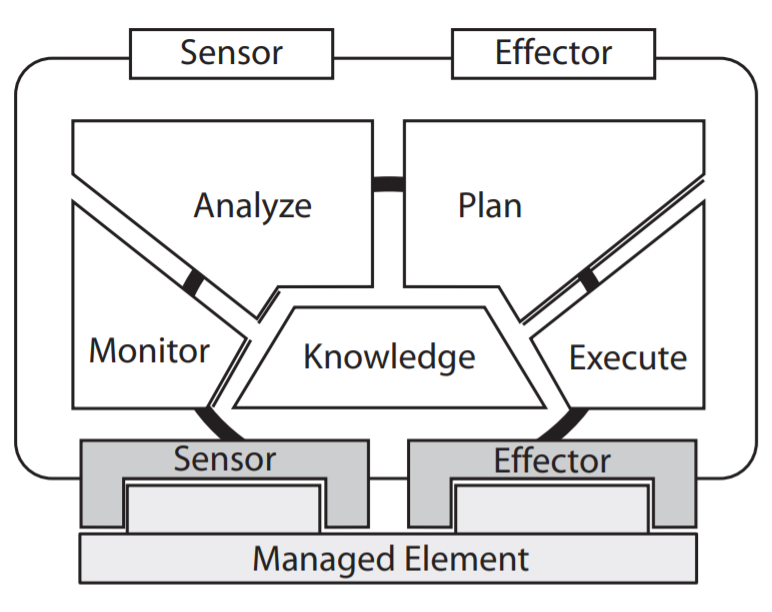
\includegraphics[scale=0.5]{images/MAPE-K.png}
\caption {Diagrama de funcionamento da arquitetura MAPE-K~\citep{Abbas_2010}.}
\label{fig:MAPEK}
\end{figure}

\subsection{\textit{Machine Learning}}
Aprendizado de Máquina (\textit{Machine Learning}, em inglês) pode ser definido como “a prática de usar algoritmos para coletar dados, aprender com eles, e então fazer uma determinação ou predição sobre alguma coisa no mundo. Em vez de implementar as rotinas de software manualmente, com um gama específica de instruções para completar uma tarefa em particular, a máquina é `treinada` usando uma quantidade grande de dados e algoritmos que dão e ela a habilidade de aprender como executar a tarefa”~\citep{Copeland_2016}, podendo ser dividido em processos de coleta, limpeza e refinamento de dados, treinamento e avaliação. As tarefas de aprendizado podem ser classificadas em três categorias básicas~\citep{MLWikipedia_2021}~\citep{MLSAS_2021}:

\begin{itemize}
\item \textbf{Aprendizado supervisionado}: O treinamento é realizado por meio de exemplos rotulados, como uma entrada na qual a saída desejada é conhecida. Através de métodos como classificação, regressão e \textit{gradient boosting}, o aprendizado supervisionado utiliza padrões para prever os valores de rótulos em dados não-rotulados adicionais. O aprendizado supervisionado é comumente empregado em aplicações nas quais dados históricos preveem eventos futuros prováveis.
\item \textbf{Aprendizado não-supervisionado}: É utilizado em dados que não possuem rótulos históricos. A “resposta certa” não é informada ao sistema, o algoritmo deve descobrir o que está sendo mostrado. O objetivo é explorar os dados e encontrar alguma estrutura dentro deles. Técnicas populares incluem mapas auto-organizáveis, mapeamento por proximidade, agrupamento \textit{k-means} e decomposição em valores singulares. Esses algoritmos também são utilizados para segmentar tópicos de texto, recomendar itens e identificar pontos discrepantes nos dados.
\item \textbf{Aprendizado por reforço}: O algoritmo descobre através de testes do tipo “tentativa e erro” quais ações rendem as maiores recompensas. Este tipo de aprendizado possui três componentes principais: o agente (o aprendiz ou tomador de decisão), o ambiente (tudo com que o agente interage) e ações (o que o agente pode fazer). O objetivo é que o agente escolha ações que maximizem a recompensa esperada em um período de tempo determinado. O agente atingirá o objetivo muito mais rápido se seguir uma boa política, então o foco do aprendizado por reforço é descobrir a melhor política.
\end{itemize}

\subsection{\textit{Fairness} em \textit{Machine Learning}}

É possível descrever o conceito de \textit{Fairness} no contexto de aprendizagem supervisionada, onde um modelo $f$ pode prever um conjunto de resultados $y$ a partir de um conjunto de \textit{features} $x$, evitando discriminação injusta em relação a um atributo protegido $a$. É permitido, mas não exigido, que $a$ seja um componente de $x$~\citep{Begley_2021}. Em outras palavras, um modelo de ML considerado justo é aquele onde a correlação de seu resultado é baixa em relação a dados de entrada considerados como sensíveis a discriminações. Algoritmos de \textit{Machine Learning} não são capazes de diferenciar contextos sociais, onde um resultado mais eficiente de acordo com os dados disponíveis podem amplificar as desigualdades sociais e tomar decisões de modo injusto~\citep{Mehrabi_2021}. Estes dados sensíveis, tendo como exemplos cor de pele, raça, sexo, idade e altura, são considerados atributos protegidos, que precisam ser classificados e processados antes da execução de um algoritmo de \textit{Machine Learning}, determinarão como o algoritmo se comportará e, consequentemente, afetará suas métricas~\citep{Mougan_2022}. Os grupos de dados provenientes destes atributos protegidos são considerados grupos protegidos, que podem ser divididos em dois grupos: o grupo privilegiado, que possui vantagens no contexto do problema, e o grupo não-privilegiado, que possui desvantagens no contexto do problema e, portanto, sujeito a discriminação.

As métricas de \textit{Fairness} diferem das métricas utilizadas para avaliação do modelo, que possuem o propósito de verificar se um modelo tem previsões confiáveis ou não. Enquanto as métricas mais tradicionais avaliam a performance do modelo e seus dados como um todo e seus resultados gerais, as métricas de \textit{Fairness} avaliam se os resultados gerais também se refletem em grupos específicos, para verificar se não há disparidade ou discriminação nos resultados propostos. Exemplos de métricas utilizadas para isso são a Taxa de Verdadeiros Positivos e a Taxa de Falsos Positivos. Enquanto a \textbf{Taxa de Verdadeiros Positivos} (TVP, ou TPR pelo termo em inglês \textbf{True Positive Rate}) é a fração de casos positivos reais (TP) de todos os casos negativos previstos incorretamente como estando na classe positiva (FN), a \textbf{Taxa de Falsos Positivos} (TFP, ou FPR pelo termo em inglês \textbf{False Positive Rate}) é a fração de casos negativos previstos incorretamente como estando na classe positiva (FP) de todos os casos positivos reais (TN):

\begin{equation}
TPR = \frac{TP}{TP + FN}
FPR = \frac{FP}{FP + TN}
\end{equation}

Dada essas métricas iniciais, considerando $Y=1$ a classe positiva, $Z=0$ o grupo não-privilegiado e $Z=1$ o grupo privilegiado, algumas das definições de \textit{Fairness} mais usadas são as seguintes:

\begin{itemize}
\item \textbf{Diferença de paridade estatística (\textit{Statistical parity difference}), ou discriminação~\citep{Zemel_2013}:} Esta métrica é baseada na seguinte fórmula:

\begin{equation}
Pr(Y=1|Z=0)-Pr(Y=1|Z=1)
\end{equation}
 
Aqui, o viés ou paridade estatística é a diferença entre a probabilidade de que um indivíduo aleatório retirado dos não-privilegiados seja rotulado como 1 e a probabilidade de que um indivíduo aleatório dos privilegiados seja rotulado como 1. Portanto, um valor próximo de 0 é considerado justo.

\item \textbf{Diferença de oportunidade igual (\textit{Equal opportunity difference})~\citep{Biswas_2020}:} É a diferença entre a taxa positiva verdadeira do grupo não privilegiado e a taxa positiva verdadeira do grupo privilegiado:

\begin{equation}
TPR_{Z=0} - TPR_{Z=1}
\end{equation}
 
Um valor próximo de 0 é considerado justo. Um classificador binário satisfaz a igualdade de oportunidades quando a taxa positiva verdadeira de ambos os grupos são iguais~\citep{Hardt_2016}

\item \textbf{Diferença de probabilidade média (\textit{Average odds difference})~\citep{Biswas_2020}:} Essa métrica usa a taxa de falsos positivos e a taxa positiva verdadeira para calcular a tendência, calculando a igualdade de probabilidades com a fórmula:

\begin{equation}
\frac{1}{2}(|FPR_{Z=0} - FPR_{Z=1}|+|TPR_{Z=0} - TPR_{Z=1}|)
\end{equation}
 
Precisa ser próximo a 0 para ser considerado justo.

\item \textbf{Impacto de disparidade (\textit{Disparate impact})~\citep{Biswas_2020}:} Para esta métrica, é usada a seguinte fórmula:

\begin{align*}
\frac{Pr(Y=1|Z=0)}{Pr(Y=1|Z=1)}
\end{align*}

Usa as mesmas probabilidades da diferença de paridade estatística, mas como é calculada como uma proporção o valor esta métrica possui um comportamento não-linear. Desta forma, um valor próximo de 1 é considerado justo.

\item \textbf{Índice de Theil (\textit{Theil index})~\citep{Speicher_2018}:} Esta medida também é conhecida como índice de entropia generalizado, mas com o valor de $\alpha$ usado neste índice igual a 1~\citep{Speicher_2018}. É calculado com a seguinte fórmula:

\begin{align*}
\frac{1}{n}\sum^{n}_{i=0}\frac{b_i}{\mu}\ln{\frac{b_i}{\mu}}
\end{align*}

Onde n é a quantidade de elementos e $b_i$ é obtido com a fórmula $b_i = \hat{y}_i - y_i + 1$. Nesta fórmula, $y_i$ é o conjunto de saídas, $\hat{y}_i$ é o conjunto de previsões dadas pelo modelo. Também precisa ser próximo a 0 para ser considerado justo.

\end{itemize}

\section{Solução Proposta}

\subsection{Arquitetura}

\begin{figure*}[h]
\centering
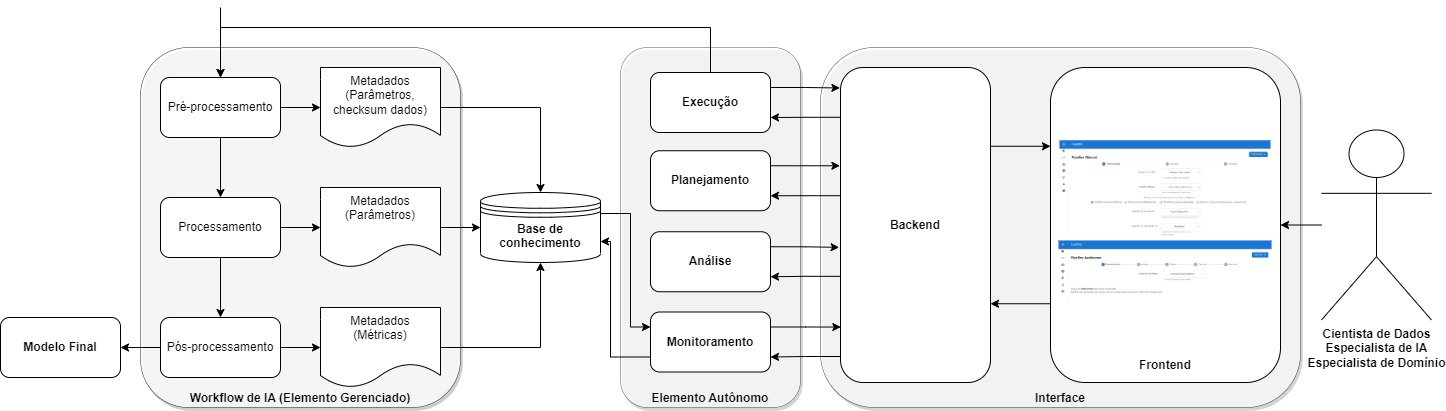
\includegraphics[scale=0.3]{images/backend-frontend-ml.jpg}
\caption {Comunicação entre Interface, gerente autonômico, Engenharia de Dados e \textit{Workflow} de IA}
\label{fig:BackendFrontendML}
\end{figure*}

O sistema implementado é dividido em 5 módulos:

\begin{itemize}
    \item {\textbf{Engenharia de Dados:}} Módulo com o objetivo de executar processos de transformação e limpeza de dados.
    \item {\textbf{Workflow de ML:}} Módulo que executa um Pipeline de uma aplicação automatizada de ML, com etapas de preparação dos dados (Pré-processamento), treinamento (Processamento) e avaliação dos resultados (Pós-processamento) para a geração de um modelo final.
    \item {\textbf{Gerenciador Autonômico:}} Módulo contendo o \textit{loop} MAPE-K que controla o Workflow como elemento gerenciado para automatizar todas as suas etapas, com o objetivo de evitar com que perca-se tempo em execuções manuais que podem demorar dependendo do algoritmo e do conjunto de dados utilizado.
    \item {\textbf{Interface (Frontend):}} Módulo criado com o objetivo de simular a etapa anterior, porém de modo a proporcionar uma experiência de usuário mais simples e intuitiva para o Cientista de Dados.
        \item {\textbf{Backend:}} Módulo criado com o objetivo de conectar o Frontend ao Gerenciador Autonômico.
\end{itemize}

A comunicação entre estes módulos está ilustrada na figura \ref{fig:BackendFrontendML}. O módulo de Engenharia de Dados seria utilizado pelo Engenheiro de Dados, que devolveria um Conjunto de Dados com os tratamentos necessários para execução dentro do \textit{Workflow}. A interface seria utilizada pelo Cientista de Dados, que determinaria as configurações necessárias para execução dos melhores \textit{Workflows} dependendo do contexto do problema. O processo que ocorre, desde a interação da interface, passando pela execução do \textit{Workflow} e chegando na obtenção dos resultados, pode ser visualizado no Diagrama de Sequência presente na figura  \ref{fig:DiagramaSequencia}.

\begin{figure*}[h]
\centering
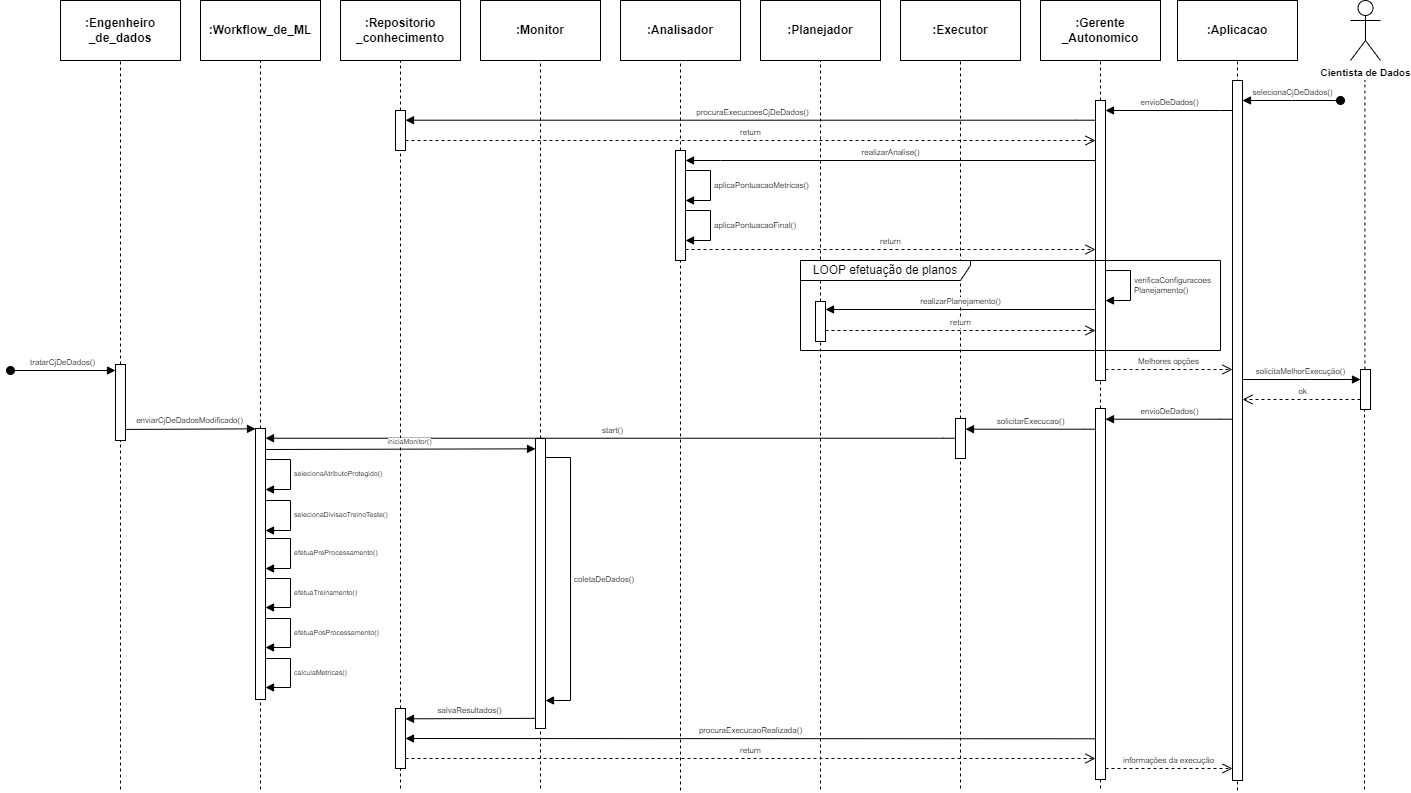
\includegraphics[scale=0.3]{images/Diagrama_Sequencia.jpg}
\caption {Diagrama de Sequência do sistema}
\label{fig:DiagramaSequencia}
\end{figure*}

\subsection{Autonomia}

Para determinar a autonomia deste workflow, o Monitor coleta os dados obtidos durante as execuções (métricas, parâmetros e etapas executadas) e os organiza para o Analisador realizar o processo de análise desses dados. Neste processo, é realizado um cálculo de pesos baseado em uma seleção livre das métricas. O motivo de existir esse cálculo é mensurar o contexto do problema de acordo com uma análise prévia do Cientista de Dados e do Especialista de Domínio, e consolidar todas as métricas para simplificar as estratégias de planejamento. As métricas são divididas em dois grupos (Métricas de Performance e Metricas de Fairness), e dentro desse grupo pode-se colocar quantas métricas forem necessárias, desde que seja respeitado o contexto de cada grupo. A cada grupo é atribuído pesos diferentes, e a cada métrica desse grupo também é atribuído pesos diferentes.

Primeiramente, é necessário padronizar as métricas de Fairness $m_{F_i}$ para $m'_{F_i}$ em um intervalo de 0 a 1, conforme apresentado na Equação \ref{eqn:normalizationFairness}. Isso garante a uniformidade dos resultados e a aplicação correta dos pesos, evitando distorções no cálculo. Como as métricas de Fairness podem envolver tanto a razão entre dois valores diferentes, como no caso da \textit{Disparate Impact}, quanto a diferença entre dois valores diferentes, como no caso da \textit{Equal Opportunity Difference}, são necessários cálculos distintos para obter esse intervalo. Como as métricas de Performance avaliadas possuem o mesmo intervalo de 0 a 1, não há necessidade de tratamento adicional para as métricas $m_{P_i}$. 

Depois, multiplica-se cada uma por seus pesos correspondentes $w_{P_i}$ e $w_{F_i}$, e realiza-se uma média ponderada dentro do grupo para atribuir uma pontuação $S_P$ para o grupo das Métricas de Performance e $S_F$ para o grupo das Metricas de Fairness, conforme exibido na equação \ref{eqn:groupScores}. Para facilitar a visualização das pontuações, multiplica-se as pontuações por um fator $X = 1000$ para o intervalo da pontuação ser de 0 a 1000 e arredonda-se o número. Após tais pontuações serem obtidas, a pontuação geral $S$ é calculada multiplicando-as por seus pesos correspondentes $w_P$ e $w_F$ e realizando a média ponderada, conforme exibido na equação \ref{eqn:totalScore}.

\begin{gather}
\label{eqn:normalizationFairness}
	m'_{F_i} = 
	\begin{cases}
	1-\lvert m_{F_i} \rvert & \text{caso $m_{F_i}$ envolva diferen\c{c}a e $-1 < m_{F_i} < 1$}\\
	0 & \text{caso $m_{F_i}$ envolva diferen\c{c}a, e $m_{F_i} >= 1$ ou $m_{F_i} <= -1$}\\
	1-\lvert \frac{1}{m_{F_i}}-1 \lvert & \text{caso $m_{F_i}$ envolva razão e $m_{F_i} > 1$}\\
	1-\lvert m_{F_i}-1 \lvert & \text{caso $m_{F_i}$ envolva razão e $m_{F_i} <= 1$}\\
	m_{F_i} & \text{caso contrário}
	\end{cases}
\end{gather}

\begin{equation}
\label{eqn:groupScores}
	\begin{aligned}
	S_F = \round{X \times \frac{\sum_{i=1}^{n_F} w_{m'_{F_i}} \times m'_{F_i}}{\sum_{i=1}^{n} w_{m'_{F_i}}}}\\
	S_P = \round{X \times \frac{\sum_{i=1}^{n_P} w_{m_{P_i}} \times m_{P_i}}{\sum_{i=1}^{n} w_{m_{P_i}}}}
	\end{aligned}
\end{equation}

\begin{equation}
\label{eqn:totalScore}
	S = \frac{w_F \times S_F + w_P \times S_P}{w_F + w_P}
\end{equation}

Para este cálculo ser realizado, é necessário como pré-requisito execuções anteriores realizadas no workflow, para que o mesmo grave as métricas necessárias e determine quais as melhores combinações através da pontuação.

\subsection{Determinação do Planejamento}

Para determinação das melhores execuções possíveis pelo Workflow, algumas estratégias foram implantadas no Planejador:

\begin{itemize}
	\item \textbf{Filtragem de algoritmos}: Alguns algoritmos podem estar mal implementados ou seus modelos podem estar com métricas que necessitam uma melhor análise do Cientista de Dados para serem consideradas confiáveis. Para isso não acontecer, é possível realizar um filtro de acordo com as combinações de algoritmos consideradas confiáveis antes de selecionar os modelos ideais.
	\item \textbf{Intervalo de resultados}: Pelo mesmo motivo da estratégia anterior, métricas com resultados não confiáveis podem causar distorções a pontuação obtida pelo cálculo realizado no processo de análise. Para amenizar esas distorções, foi criado um intervalo de pontuação mínimo e máximo para determinar pontuações que podem ser consideradas confiáveis para avaliação.
\end{itemize}

Após a realização destas estratégias, o Planejador retornará as 5 melhores pontuações para o Cientista de Dados escolher, e solicitará ao Executor uma nova execução do Workflow após a escolha.

\section{Avaliação da Solução}

Foram realizados 3 Estudos de Caso para determinar a viabilidade da solução, manutenções futuras e viabilidade do Gerenciador Autonômico na escolha de melhores opções em diferentes contextos. Em todos eles, o objetivo foi a obtenção de uma classificação de crédito (boa ou ruim), através de uma série de \textit{features} e utilizando diferentes conjuntos de dados. No caso de alterações no sistema, também foram contadas as linhas de código realizadas em cada alteração, para definir se tais alterações são simples de serem feitas.

A execução para determinar as melhores opções foi realizada com 3 pesagens diferentes na pontuação geral:

\begin{itemize}
\item 50\% para métricas de Performance e 50\% para métricas de Fairness, para uma configuração equilibrada.
\item 75\% para métricas de Performance e 25\% para métricas de Fairness, para uma configuração que prioriza a performance em detrimento da justiça.
\item 25\% para métricas de Performance e 75\% para métricas de Fairness, para uma configuração que prioriza a justiça em detrimento da performance.
\end{itemize}

Todas as execuções foram realizadas utilizando uma base de conhecimento contendo cerca de 650 execuções prévias com diversas opções de conjuntos de dados, atributos protegidos e algoritmos, e são utilizadas as métricas Acurácia, Precisão, \textit{Recall}, \textit{F1-Score} e AUC como métricas de Performance e as métricas \textit{Statistical Parity Difference}, \textit{Equal Opportunity Difference}, \textit{Average Odds Difference}, \textit{Disparate Impact} e \textit{Theil Index} como métricas de \textit{Fairness}, todas com pesagens iguais em seu respectivo agrupamento.

No \textit{workflow}, foram implementados os algoritmos \textit{Disparate Impact Remover}~\citep{Feldman_2015}, \textit{Learning Fair Representations}~\citep{Zemel_2013}, \textit{Reweighing}~\citep{Kamiran_2011} e \textit{Optimized Preprocessing}~\citep{Calmon_2017} na etapa de Pré-Processamento, os algoritmos Regressão Logística, \textit{Gradient Boosting}, \textit{Random Forest}, \textit{Support Vector Machines}, \textit{Adversarial Debiasing}~\citep{Zhang_2018}, \textit{Exponentiated Gradient Reduction}~\citep{Agarwal_2018}, \textit{Grid Search Reduction}~\citep{Agarwal_2019}, \textit{Meta Fair Classifier}~\citep{Celis_2019}, \textit{Prejudice Remover}~\citep{Kamishima_2012} e \textit{Rich Subgroup Fairness}~\citep{Kearns_2018} na etapa de Processamento, e os algoritmos \textit{Equalized Odds}~\citep{Hardt_2016}, \textit{Calibrated Equalized Odds}~\citep{Pleiss_2017} e \textit{Reject Option Classification}~\citep{Kamiran_2012} na etapa de Pós-Processamento. Como não foram encontrados estudos onde são utilizados redução de viés em mais de uma etapa do processo de \textit{Machine Learning}, é realizada a execução de apenas um algoritmo de redução de viés por \textit{workflow}. Por apresentarem dados considerados não confiáveis, foram filtrados as execuções com os algoritmos \textit{Optimized Preprocessing} e \textit{Reject Option Classification}, que correspondiam cerca de 5\% do total da base utilizada.

\subsection{Estudo de Caso 1: Viabilidade e utilidade do Gerenciador Autonômico}

 Neste Estudo de Caso, o foco foi colocado em testar e verificar como o Gerenciador Autonômico se comporta em um cenário com diversas execuções prévias do Workflow, utilizando o German Credit Dataset~\citep{ucigerman_2021} como conjunto de dados, Idade e Nacionalidade como opções de atributos protegidos e um intervalo de pontuação entre 500 e 950. Os resultados estão presentes abaixo nas Tabelas \ref{tbl:ScoreMAPEKGeral5050}, \ref{tbl:ScoreMAPEKGeral7525} e \ref{tbl:ScoreMAPEKGeral2575}:

\begin{table}[H]
\begin{center}
  \caption{Melhores opções escolhidas pelo Gerenciador Autonômico \\ Todos os métodos - 50\% Performance/50\% Fairness}
\label{tbl:ScoreMAPEKGeral5050}
  \resizebox{\linewidth}{!}{%
\begin{tabular}{c|c|c|c|c|c|c}
\multicolumn{4}{c|}{Workflow} & \multicolumn{3}{c}{Pontuação} \\
\hline
Atributo protegido & Pré-processamento & Treinamento & Pós-processamento & Performance & Fairness & \textbf{Geral} \\
\hline
Idade & Nenhum & Regressão Logística & Equalized Odds & 968 & 860 & \textbf{914} \\
Nacionalidade & Nenhum & Random Forest & Calibrated Equalized Odds & 902 & 922 & \textbf{912} \\
Nacionalidade & Nenhum & Gradient Boosting & Calibrated Equalized Odds & 870 & 925 & \textbf{898} \\
Idade & Nenhum & Gradient Boosting & Equalized Odds & 927 & 862 & \textbf{894} \\
Idade & Reweighing & Gradient Boosting & Nenhum & 804 & 931 & \textbf{868} \\
\end{tabular}}
\end{center}
\end{table}

\begin{table}[H]
\begin{center}
  \caption{Melhores opções escolhidas pelo Gerenciador Autonômico \\ Todos os métodos - 75\% Performance/25\% Fairness}
\label{tbl:ScoreMAPEKGeral7525}
  \resizebox{\linewidth}{!}{%
\begin{tabular}{c|c|c|c|c|c|c}
\multicolumn{4}{c|}{Workflow} & \multicolumn{3}{c}{Pontuação} \\
\hline
Atributo protegido & Pré-processamento & Treinamento & Pós-processamento & Performance & Fairness & \textbf{Geral} \\
\hline
Idade & Nenhum & Regressão Logística & Equalized Odds & 968 & 860 & \textbf{941} \\
Idade & Nenhum & Gradient Boosting & Equalized Odds & 927 & 862 & \textbf{910} \\
Nacionalidade & Nenhum & Random Forest & Calibrated Equalized Odds & 902 & 922 & \textbf{907} \\
Nacionalidade & Nenhum & Gradient Boosting & Calibrated Equalized Odds & 870 & 925 & \textbf{883} \\
Idade & Nenhum & Random Forest & Equalized Odds & 898 & 799 & \textbf{874} \\
\end{tabular}}
\end{center}
\end{table}

\begin{table}[H]
\begin{center}
  \caption{Melhores opções escolhidas pelo Gerenciador Autonômico \\ Todos os métodos - 25\% Performance/75\% Fairness}
\label{tbl:ScoreMAPEKGeral2575}
  \resizebox{\linewidth}{!}{%
\begin{tabular}{c|c|c|c|c|c|c}
\multicolumn{4}{c|}{Workflow} & \multicolumn{3}{c}{Pontuação} \\
\hline
Atributo protegido & Pré-processamento & Treinamento & Pós-processamento & Performance & Fairness & \textbf{Geral} \\
\hline
Idade & Disparate Impact Remover & Support Vector Machines & Nenhum & 747 & 989 & \textbf{928} \\
Nacionalidade & Disparate Impact Remover & Support Vector Machines & Nenhum & 747 & 989 & \textbf{928} \\
Idade & Nenhum & Adversarial Debiasing & Nenhum & 742 & 979 & \textbf{920} \\
Nacionalidade & Reweighing & Support Vector Machines & Nenhum & 755 & 972 & \textbf{918} \\
Nacionalidade & Learning Fair Representations & Support Vector Machines & Nenhum & 755 & 972 & \textbf{918} \\
\end{tabular}}
\end{center}
\end{table}

Nessas execuções, surpreende 2 observações. A primeira é o fato da predominância de algoritmos com redução de viés no pós-processamento/resultado especialmente em configurações que priorizavam performance, contrariando o esperado de que os algoritmos com redução de viés aumentavam justiça em detrimento da performance. A segunda é a predominância de algoritmos com redução de viés no pré-processamento/dado em configurações que priorizavam justiça, principalmente pois todas as execuções usavam \textit{Support Vector Machines} como algoritmo de treinamento.

Em todas as execuções, foi possível perceber que a escolha do \textit{workflow} com o melhor equilíbrio entre estes dois grupos de métricas com contextos completamente diferentes ainda se torna difuso diante da grande quantidade de métricas e conjuntos de algoritmos utilizados. Além disso, a diferença entre as métricas é extremamente pequena e dificulta ainda mais a escolha. Nesse contexto, a consolidação das métricas em grupos simplifica a visualização de quais \textit{workflows} são mais equilibrados, e o uso de pesos para cada métrica e para cada grupo pode calibrar qual o melhor equilíbrio desejado para determinada situação. Deste modo, pode-se concluir também que, em um contexto de desenvolvimento, o processo simplifica a decisão do Cientista de Dados e reduz significantemente o tempo para obtenção e implantação de um modelo otimizado, pois não exigirá execuções em diversos algoritmos uma vez que já há uma base de conhecimento prévia. Além disso, poderá poupar processamento e custos para a resolução de diversos outros problemas, uma vez que as execuções economizadas pelas equipes que utilizariam esse processo abrem margem para que outras equipes utilizem esse processamento.

\subsection{Estudo de Caso 2: Evolução do \textit{Workflow} adicionando um novo conjunto de dados}

Neste Estudo de Caso, foi realizada uma evolução do sistema adicionando um novo conjunto de dados mais próximo de conjuntos de dados reais. Além de reforçar a versatilidade do Gerenciador Autonômico em diferentes contextos, um maior foco foi colocado na manutenção do sistema, discutindo se as etapas e arquiteturas escolhidas são viáveis para evoluir e manter o \textit{Workflow} sem grandes deteriorações nas ideias originais de seu desenvolvimento, desta vez utilizando o Lendingclub Dataset~\citep{lendingclub_2022} como conjunto de dados, Renda como atributo protegido e um intervalo de pontuação entre 500 e 980. Os resultados estão presentes abaixo nas Tabelas \ref{tbl:ScoreMAPEKLendingclubGeral5050}, \ref{tbl:ScoreMAPEKLendingclubGeral7525} e \ref{tbl:ScoreMAPEKLendingclubGeral2575}:

\begin{table}[H]
\begin{center}
  \caption{Melhores opções escolhidas pelo Gerenciador Autonômico \\ Todos os métodos - 50\% Performance/50\% Fairness}
\label{tbl:ScoreMAPEKLendingclubGeral5050}
  \resizebox{\linewidth}{!}{%
\begin{tabular}{c|c|c|c|c|c|c}
\multicolumn{4}{c|}{Workflow} & \multicolumn{3}{c}{Pontuação} \\
\hline
Atributo protegido & Pré-processamento & Treinamento & Pós-processamento & Performance & Fairness & \textbf{Geral} \\
\hline
Renda & Learning Fair Representations & Random Forest & Nenhum & 991 & 968 & \textbf{979} \\
Renda & Nenhum & Gradient Boosting & Equalized Odds & 988 & 969 & \textbf{978} \\
Renda & Reweighing & Random Forest & Nenhum & 991 & 963 & \textbf{977} \\
Renda & Learning Fair Representations & Regressão Logística & Nenhum & 981 & 973 & \textbf{977} \\
Renda & Reweighing & Gradient Boosting & Nenhum & 987 & 964 & \textbf{976} \\
\end{tabular}}
\end{center}
\end{table}

\begin{table}[H]
\begin{center}
  \caption{Melhores opções escolhidas pelo Gerenciador Autonômico \\ Todos os métodos - 75\% Performance/25\% Fairness}
\label{tbl:ScoreMAPEKLendingclubGeral7525}
  \resizebox{\linewidth}{!}{%
\begin{tabular}{c|c|c|c|c|c|c}
\multicolumn{4}{c|}{Workflow} & \multicolumn{3}{c}{Pontuação} \\
\hline
Atributo protegido & Pré-processamento & Treinamento & Pós-processamento & Performance & Fairness & \textbf{Geral} \\
\hline
Renda & Nenhum & Regressão Logística & Equalized Odds & 985 & 965 & \textbf{980} \\
Renda & Learning Fair Representations & Gradient Boosting & Nenhum & 987 & 960 & \textbf{980} \\
Renda & Learning Fair Representations & Regressão Logística & Nenhum & 981 & 973 & \textbf{979} \\
Renda & Nenhum & Grid Search Reduction & Nenhum & 989 & 950 & \textbf{979} \\
Renda & Reweighing & Regressão Logística & Nenhum & 981 & 965 & \textbf{977} \\
\end{tabular}}
\end{center}
\end{table}

\begin{table}[H]
\begin{center}
  \caption{Melhores opções escolhidas pelo Gerenciador Autonômico \\ Todos os métodos - 25\% Performance/75\% Fairness}
\label{tbl:ScoreMAPEKLendingclubGeral2575}
  \resizebox{\linewidth}{!}{%
\begin{tabular}{c|c|c|c|c|c|c}
\multicolumn{4}{c|}{Workflow} & \multicolumn{3}{c}{Pontuação} \\
\hline
Atributo protegido & Pré-processamento & Treinamento & Pós-processamento & Performance & Fairness & \textbf{Geral} \\
\hline
Renda & Learning Fair Representations & Regressão Logística & Nenhum & 981 & 973 & \textbf{975} \\
Renda & Nenhum & Gradient Boosting & Equalized Odds & 988 & 969 & \textbf{974} \\
Renda & Learning Fair Representations & Random Forest & Nenhum & 991 & 968 & \textbf{973} \\
Renda & Nenhum & Exponentiated Gradient Reduction & Nenhum & 986 & 966 & \textbf{971} \\
Renda & Reweighing & Gradient Boosting & Nenhum & 987 & 964 & \textbf{970} \\
\end{tabular}}
\end{center}
\end{table}

Nessas execuções, a principal observação notada é que a relação de algoritmos com melhores desempenhos mudou completamente, com predominância do algoritmo \textit{Learning Fair Representations} para redução de viés e Regressão Logística para algoritmo de treinamento. Também se nota que algoritmos com redução de viés no pós-processamento e algoritmos de treinamento como \textit{Support Vector Machines} não foram tão eficientes. Com isso, pode-se concluir que, ao mudar o contexto do problema e os dados envolvidos, o Gerenciador Autonômico pode ajudar a enxergar tais sutilezas e ajudar em uma decisão de forma mais eficiente e ágil. Entretanto, os dados e metadados obtidos não ajudaram a entender o porquê de tais sutilezas acontecerem.

Para processar o Lendingclub Dataset, foram necessárias modificações para realizar a evolução do sistema e adicionar este conjunto de dados como opção no \textit{Workflow}. Estas foram contadas de acordo com seus \textit{commits} realizados no repositório e exibidos  na Tabela \ref{tbl:ManutencaoPipelineDataset}:

\begin{table}[H]
\begin{center}
  \caption{Quantidade de modificações realizadas ao adicionar um novo conjunto de dados ao \textit{Workflow}}
\label{tbl:ManutencaoPipelineDataset}
  \resizebox{\linewidth}{!}{%
{\def\arraystretch{1.5}
\begin{tabular}{c|c|c|c|c|c|c}
Parte do Sistema & \makecell{Linhas alteradas} & Total de linhas & \makecell{Arquivos alterados} & Total de arquivos & \makecell{\% linhas alteradas} & \makecell{\% arquivos alterados} \\
\hline
\makecell{Engenharia de Dados} & 122 & 277 & 2 & 3 & \textbf{44,04\%} & \textbf{66,67\%} \\
\textit{Workflow} de ML & 76 & 1982 & 5 & 38 & \textbf{3,84\%} & \textbf{13,16\%} \\
Gerenciador Autonômico & 0 & 457 & 0 & 10 & \textbf{0,00\%} & \textbf{0,00\%} \\
\makecell{Interface} & 13 & 2905 & 2 & 14 & \textbf{0,45\%} & \textbf{14,29\%} \\
\makecell{\textit{Backend}} & 4 & 432 & 1 & 7 & \textbf{0,93\%} & \textbf{14,29\%} \\
\hline
\textbf{TOTAL} & \textbf{215} & \textbf{6053} & \textbf{10} & \textbf{72} & \textbf{3,55\%} & \textbf{13,89\%} \\
\end{tabular}}}
\end{center}
\end{table}

A adição do conjunto de dados não exigiu modificações no Gerenciador Autonômico, mesmo os resultados sendo completamente diferentes do Estudo de Caso anterior. Isto reforça a autonomia proposta no \textit{loop} MAPE-K, possibilitando escolhas diferentes baseadas nos metadados presentes no \textit{Workflow} sem realizar modificações. O Gerenciador Autonômico só exigirá modificações se os metadados salvos do \textit{Workflow} forem modificados, ou se modificar alguma configuração intrínseca ao próprio Gerenciador, que é desacoplado do \textit{Workflow}. 

Os elementos na Interface exigiram pouquíssimas modificações, podendo ser resumidos a simples adições para disponibilizar a opção do novo conjunto de dados ao Cientista de Dados. As maiores modificações foram realizadas no \textit{Workflow} de ML e nas Transformações do Conjunto de Dados, principalmente deste último. Das modificações no \textit{Workflow} de ML, a grande parte (34 linhas, ou 44,74\% das linhas) foi realizada no pré-processamento do dado para o cálculo dos algoritmos de treinamento. Embora a estruturação baseada na arquitetura \textit{Pipes-and-Filters} exija a criação de classes adicionais para o \textit{workflow} (2 para pipes e 1 para filtro), é nas etapas de processamento e transformação dos dados que os Engenheiros e Cientistas de Dados vão gastar a maior parte do tempo e fazer mais modificações.

Embora o uso da arquitetura \textit{Pipes-and-Filters} exija a escrita de algumas linhas a mais, ela permite encapsular os algoritmos e separar os interesses de forma simples, tornando possível ter um bom \textit{Design} do código. Isso torna a manutenção/evolução do sistema no \textit{Workflow} e na Interface relativamente simples, desde que o desenvolvedor saiba em quais arquivos as modificações serão realizadas. Por isso, a criação de uma documentação é extremamente importante para que um novo desenvolvedor entenda o sistema como um todo e não adicione linhas de forma desnecessária.

\subsection{Estudo de Caso 3: Evolução do \textit{Workflow} com desenvolvedor sem conhecimento anterior adicionando um novo algoritmo de treinamento}

Neste Estudo de Caso, realizou-se uma evolução do sistema adicionando um novo algoritmo de classificação. Novamente é discutida a manutenção do sistema, desta vez com foco nas decisões de outros desenvolvedores. Para isso, foi verificado se as arquiteturas escolhidas são versáteis e simples o suficiente para que novos desenvolvedores possam entender o contexto do sistema e realizar novas evoluções com facilidade, novamente utilizando o Lendingclub Dataset~\citep{lendingclub_2022} como conjunto de dados, Renda como atributo protegido e um intervalo de pontuação entre 500 e 980. 

Durante uma sessão de desenvolvimento com um outro desenvolvedor, com duração de cerca de 1 e 2 horas, um novo algoritmo de classificação foi adicionado à estrutura do \textit{workflow} por ele utilizando a documentação elaborada durante o Estudo de Caso anterior. Durante a sessão, alguns itens como erros na documentação e bugs foram notados e corrigidos, através de observação e \textit{feedbacks} do desenvolvedor. Devido a esses problemas, uma pequena parte da sessão foi dedicada em auxílios e dúvidas para que o desenvolvedor evitasse perder tempo com eles e se concentrasse no desenvolvimento do \textit{workflow}. Depois da sessão, o desenvolvedor preencheu um questionário indicando um perfil com certa experiência na área de dados e desenvolvimento, com impressões positivas da sessão e uma implementação sem dificuldades. Embora a intenção inicial era que o desenvolvedor apenas se guiasse pela documentação, ele próprio considerou a adaptação a tal experimento rápida, independente do auxílio fornecido. Isso sugere que as decisões iniciais tomadas na implementação foram corretas e facilitaram o desenvolvimento de evoluções.

O algoritmo de classificação escolhido para o desenvolvimento foi o Naive Bayes~\citep{Naive_Bayes_2004}, que também é bastante difundido como classificador. Após o desenvolvimento, os resultados estão presentes abaixo nas Tabelas \ref{tbl:ScoreMAPEKLendingclubCaso35050}, \ref{tbl:ScoreMAPEKLendingclubCaso37525} e \ref{tbl:ScoreMAPEKLendingclubCaso32575}:

\begin{table}[H]
\begin{center}
  \caption{Melhores opções escolhidas pelo Gerenciador Autonômico \\ Todos os métodos - 50\% Performance/50\% Fairness}
\label{tbl:ScoreMAPEKLendingclubCaso35050}
  \resizebox{\linewidth}{!}{%
\begin{tabular}{c|c|c|c|c|c|c}
\multicolumn{4}{c|}{Workflow} & \multicolumn{3}{c}{Pontuação} \\
\hline
Atributo protegido & Pré-processamento & Treinamento & Pós-processamento & Performance & Fairness & \textbf{Geral} \\
\hline
Renda & Learning Fair Representations & Random Forest & Nenhum & 991 & 968 & \textbf{979} \\
Renda & Nenhum & Gradient Boosting & Equalized Odds & 988 & 969 & \textbf{978} \\
Renda & Reweighing & Random Forest & Nenhum & 991 & 963 & \textbf{977} \\
Renda & Learning Fair Representations & Regressão Logística & Nenhum & 981 & 973 & \textbf{977} \\
Renda & Reweighing & Gradient Boosting & Nenhum & 987 & 964 & \textbf{976} \\
\end{tabular}}
\end{center}
\end{table}

\begin{table}[H]
\begin{center}
  \caption{Melhores opções escolhidas pelo Gerenciador Autonômico \\ Todos os métodos - 75\% Performance/25\% Fairness}
\label{tbl:ScoreMAPEKLendingclubCaso37525}
  \resizebox{\linewidth}{!}{%
\begin{tabular}{c|c|c|c|c|c|c}
\multicolumn{4}{c|}{Workflow} & \multicolumn{3}{c}{Pontuação} \\
\hline
Atributo protegido & Pré-processamento & Treinamento & Pós-processamento & Performance & Fairness & \textbf{Geral} \\
\hline
Renda & Nenhum & Regressão Logística & Equalized Odds & 985 & 965 & \textbf{980} \\
Renda & Learning Fair Representations & Gradient Boosting & Nenhum & 987 & 960 & \textbf{980} \\
Renda & Learning Fair Representations & Regressão Logística & Nenhum & 981 & 973 & \textbf{979} \\
Renda & Nenhum & Grid Search Reduction & Nenhum & 989 & 950 & \textbf{979} \\
Renda & Reweighing & Regressão Logística & Nenhum & 981 & 965 & \textbf{977} \\
\end{tabular}}
\end{center}
\end{table}

\begin{table}[H]
\begin{center}
  \caption{Melhores opções escolhidas pelo Gerenciador Autonômico \\ Todos os métodos - 25\% Performance/75\% Fairness}
\label{tbl:ScoreMAPEKLendingclubCaso32575}
  \resizebox{\linewidth}{!}{%
\begin{tabular}{c|c|c|c|c|c|c}
\multicolumn{4}{c|}{Workflow} & \multicolumn{3}{c}{Pontuação} \\
\hline
Atributo protegido & Pré-processamento & Treinamento & Pós-processamento & Performance & Fairness & \textbf{Geral} \\
\hline
Renda & Nenhum & Naive Bayes & Calibrated Equalized Odds & 991 & 976 & \textbf{980} \\
Renda & Learning Fair Representations & Regressão Logística & Nenhum & 981 & 973 & \textbf{975} \\
Renda & Nenhum & Gradient Boosting & Equalized Odds & 988 & 969 & \textbf{974} \\
Renda & Learning Fair Representations & Random Forest & Nenhum & 991 & 968 & \textbf{973} \\
Renda & Nenhum & Exponentiated Gradient Reduction & Nenhum & 986 & 966 & \textbf{971} \\
\end{tabular}}
\end{center}
\end{table}

Para o contexto do Lendingclub Dataset a adição do Naive Bayes no \textit{workflow} mostrou seu valor, apresentando uma pontuação acima do esperado para configurações que privilegiam justiça e só não foi mais destacada por causa do limiar máximo estabelecido de 980. Entretanto, como já visto em estudos de caso anteriores, pode não funcionar em outros contextos e os dados e metadados estabelecidos não definem explicações do porquê o Naive Bayes teve um comportamento positivo para este conjunto de dados.

As evoluções realizadas no \textit{Workflow} para adicionar o Naive Bayes foram contadas de acordo com seus \textit{commits} realizados no repositório e exibidos  na Tabela \ref{tbl:ManutencaoPipelineDataset}:

\begin{table}[H]
\begin{center}
  \caption{Quantidade de modificações realizadas ao adicionar um novo algoritmo ao \textit{Workflow}}
\label{tbl:ManutencaoPipelineCaso3}
  \resizebox{\linewidth}{!}{%
{\def\arraystretch{1.5}
\begin{tabular}{c|c|c|c|c|c|c}
Parte do Sistema & \makecell{Linhas alteradas} & Total de linhas & \makecell{Arquivos alterados} & Total de arquivos & \makecell{\% linhas alteradas} & \makecell{\% arquivos alterados} \\
\hline
\makecell{Engenharia de Dados} & 0 & 277 & 0 & 3 & \textbf{0,00\%} & \textbf{0,00\%} \\
\textit{Workflow} de ML & 60 & 2042 & 5 & 39 & \textbf{2,94\%} & \textbf{12,82\%} \\
Gerenciador Autonômico & 1 & 458 & 1 & 10 & \textbf{0,22\%} & \textbf{10,00\%} \\
\makecell{Interface} & 71 & 2948 & 3 & 14 & \textbf{2,41\%} & \textbf{21,43\%} \\
\makecell{\textit{Backend}} & 1 & 433 & 1 & 7 & \textbf{0,23\%} & \textbf{14,29\%} \\
\hline
\textbf{TOTAL} & \textbf{132} & \textbf{6157} & \textbf{9} & \textbf{72} & \textbf{2,14\%} & \textbf{12,50\%} \\
\end{tabular}}}
\end{center}
\end{table}

Desta vez, o único módulo sem necessidade de modificações foi Engenharia de Dados, por já terem sido implementadas anteriormente. Também, a única modificação necessária no Gerenciador Autonômico e no \textit{Backend} foi a adição do Naive Bayes como parte de uma parametrização, que poderia ser transferida para um arquivo externo de configuração e não exigir modificações futuramente via código.

No geral, foram exigidas menos modificações que a evolução proposta no Estudo de Caso anterior. A única parte que exigiu mais modificações foi na Interface, em grande parte por causa de um único componente presente na tela de Configurações para Planejamento do Gerenciador Autonômico. Fora esta exceção, adicionar um algoritmo é uma evolução mais simples de ser feita, e junto com a documentação criada um desenvolvedor com relativa experiência consegue executar essa tarefa sem grandes dificuldades.

\section{Conclusões e Trabalhos Futuros}

A literatura revisada sobre \textit{Fairness} verifica apenas problemas de classificação binária, e para evoluções e novos métodos é provável que ocorram refatorações no \textit{workflow}. Com a arquitetura \textit{Pipes-and-Filters}, foi possível encapsular todos os procedimentos presentes em um \textit{workflow} de uma aplicação de \textit{Machine Learning} em etapas coesas e trocá-las caso haja a necessidade de teste com outro algoritmo, atributo protegido ou conjunto de dados, e facilitar o entendimento de outros desenvolvedores. 

Com a arquitetura MAPE-K, foi possível realizar um fluxo para que os dados obtidos no \textit{workflow} fossem analisados para facilitar uma tomada de decisão. Embora a autonomia seja viável, a supervisão humana é necessária devido a problemas ainda enfrentados pelo tema \textit{Fairness}, onde o contexto social do problema é de extrema importância ao avaliar se o modelo é considerado bom ou não. O uso de pesos para as métricas e diferentes estratégias nas fases de análise e planejamento do Gerenciador Autonômico garantem o balanceamento performance/\textit{Fairness} e ajudam a definir o contexto para uma avaliação, mas ainda depende de um Cientista de Dados e/ou de um especialista de Domínio entender quais as necessidades do problema analisado e se os resultados são aceitáveis para a publicação de um modelo otimizado e justo.

Dadas estas observações, pode-se dizer este conjunto se adaptou muito bem na implementação dos objetivos principais. Como trabalhos futuros, é possível trabalhar com algumas possibilidades. No Gerenciador Autonômico, o Analisador pode realizar uma análise mais profunda aumentando o número de indicadores e considerando grupos além de métricas de \textit{Fairness} e métricas de Performance. No \textit{workflow}, introduzir técnicas para melhora dos resultados como \textit{Data Augmentation} e \textit{K-Fold Cross-Validation}. Também é possível mudar o foco para solucionar problemas de MLOps, utilizando o sistema para determinar um melhor deploy em caso de piora nas métricas de um modelo já utilizado por clientes.

% As referências:
\bibliographystyle{plainnat}
\bibliography{full,article}

\end{document}
